\documentclass[tikz,border=10pt]{standalone}
\usetikzlibrary{calc}
\begin{document}
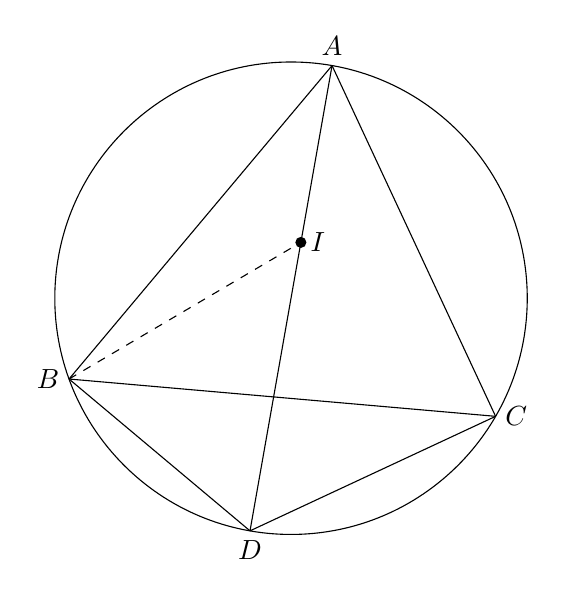
\begin{tikzpicture}
    % Define coordinates based on visual inspection
    % Circle radius approx 3cm
    \coordinate (A) at (80:3);
    \coordinate (B) at (200:3);
    \coordinate (C) at (330:3);
    \coordinate (D) at (260:3);
    
    % Point I lies on the segment AD. 
    % Visually it is about 35-40% of the way from A to D.
    \coordinate (I) at ($(A)!0.38!(D)$);
    
    % Draw the circle
    \draw (0,0) circle (3);
    
    % Draw solid edges
    \draw (A) -- (B);
    \draw (A) -- (C);
    \draw (A) -- (D);
    \draw (B) -- (C);
    \draw (B) -- (D);
    \draw (C) -- (D);
    
    % Draw dashed edge
    \draw[dashed] (B) -- (I);
    
    % Draw point I
    \fill (I) circle (2pt);
    
    % Labels
    \node[above] at (A) {$A$};
    \node[left] at (B) {$B$};
    \node[right] at (C) {$C$};
    \node[below] at (D) {$D$};
    \node[right] at (I) {$I$};
\end{tikzpicture}
\end{document}
